% !TEX root = ../../../main.tex
% 来源：中学数学实验教材·第一册（代数）
% 章节：代数运算的初步应用 / 待定系数法
% 原始文件：7.tex，行 823-851
% 类型：tikz
% ---
  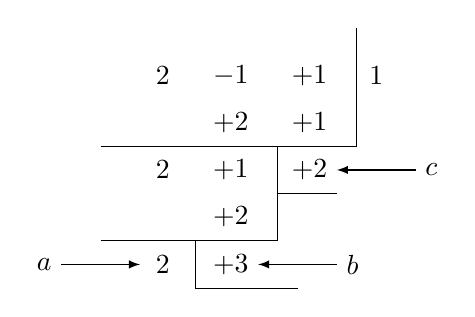
\begin{tikzpicture}[yscale=1.2, >=latex]
    \foreach \x /\xtext in {0/2,1/-1,2/+1}
    {
        \node at (\x,2)[left] {$\xtext$};
    }
    
    \foreach \x /\xtext in {1/+2,2/+1}
    {
        \node at (\x,1.5)[left] {$\xtext$};
    }
    
    \foreach \x /\xtext in {0/2,1/+1,2/+2}
    {
        \node at (\x,1)[left] {$\xtext$};
    }
    \foreach \x /\xtext in {0/2,1/+3}
    {
        \node at (\x,0)[left] {$\xtext$};
    }
    
    \node at (1,.5)[left]{$+2$}; \node at (2.5,2){1};
    \draw (-1,.25)--(1.25,.25)--(1.25,1.25);
    \draw (.2,.25)--(.2,-.25)--(1.5,-.25);
    \draw (-1,1.25)--(2.25,1.25)--(2.25,2.5);
    \draw (1.25,-.25+1)--(2,-.25+1);
    \draw [->] (3,1)node[right]{$c$}--(2,1);
    \draw [->] (2,0)node[right]{$b$}--(1,0);
    \draw [->] (-1.5,0)node[left]{$a$}--(-.5,0);
    \end{tikzpicture}
